%&tex

\chapter{Object Shape Learning}
\begin{comment}
	% PENN SHAPES
	\begin{figure}[htp]
		\begin{subfigure}{1.\textwidth}
		\centering
		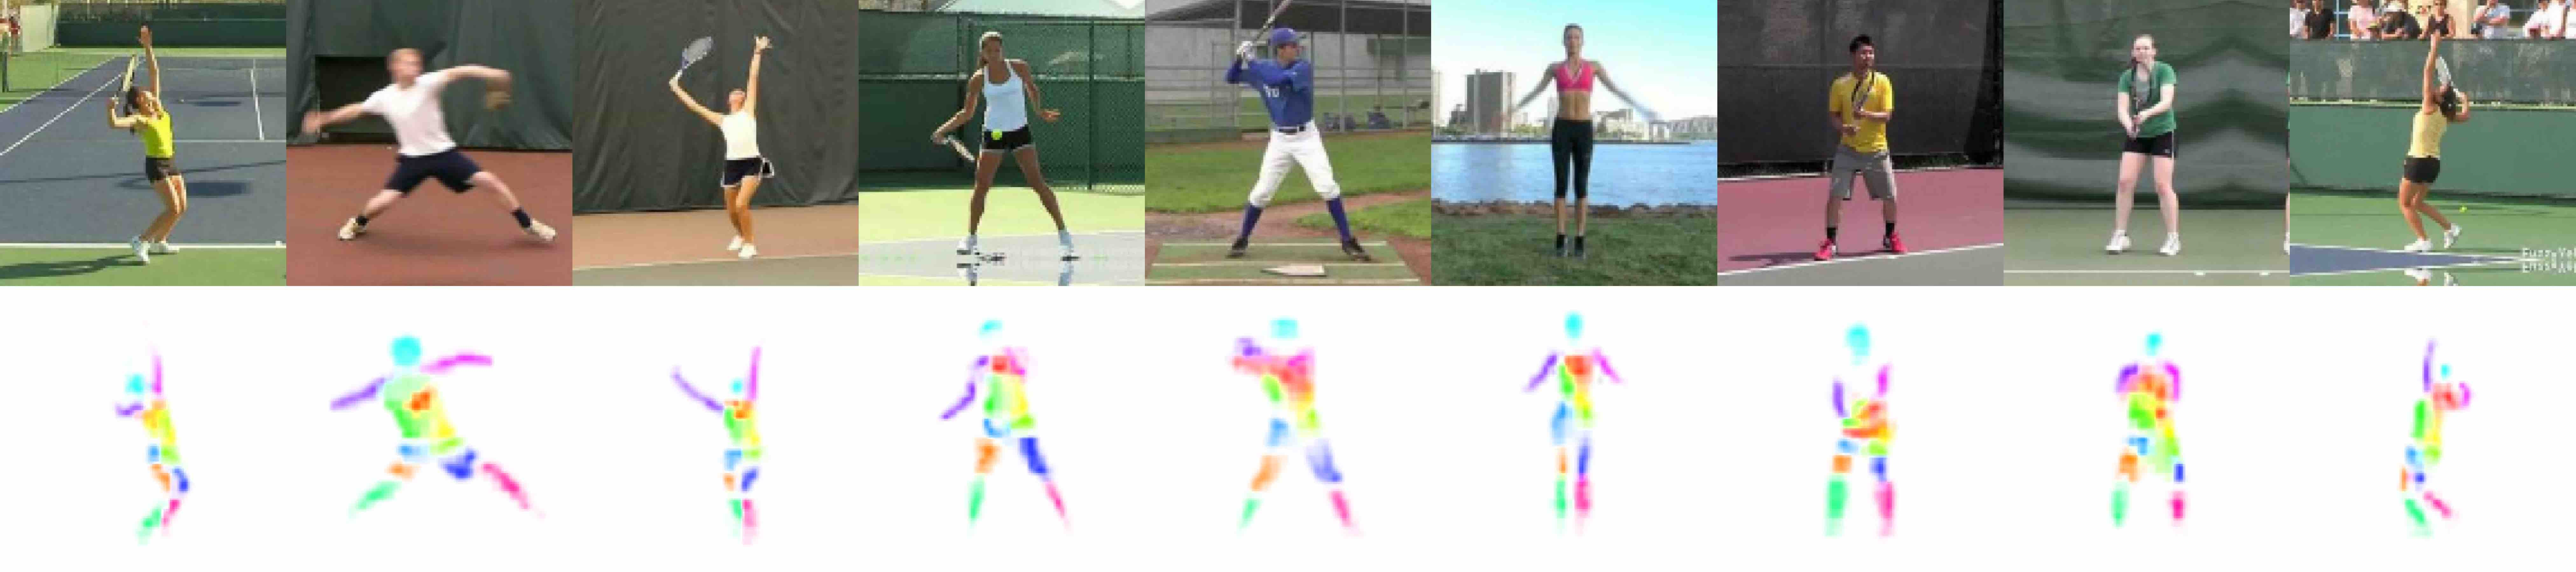
\includegraphics[trim={0cm 0cm 0cm 0cm},clip, width=1.\linewidth]{fig/shape/shape8white}\caption{}
		\label{fig:shape_penn}
		\end{subfigure}
		\begin{subfigure}{1.\textwidth}
		\centering
		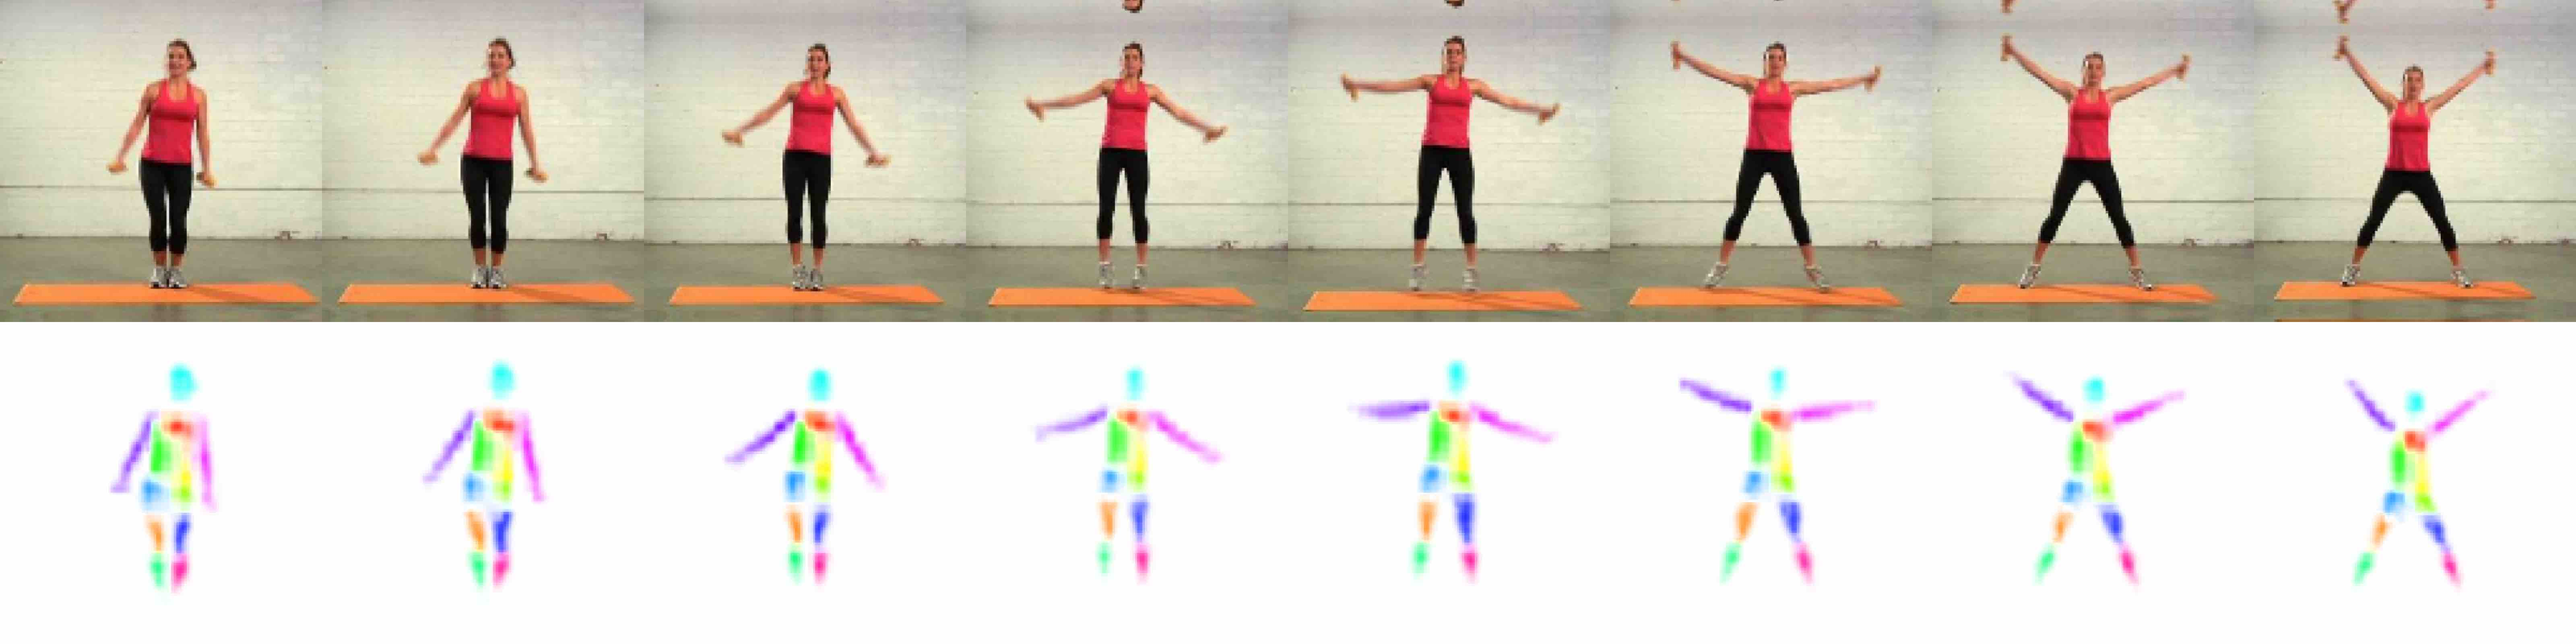
\includegraphics[trim={0cm 0cm 0cm 0cm},clip, width=1.\linewidth]{fig//shape/shape_yoga8}\caption{}
		\label{fig:shape_tennis}
		\end{subfigure}
		\caption{Learned shape representation on Penn Action. For visualization, 13 of 16 part activation maps are plotted in one image. (a) Different instances, showing intra-class consistency and (b) video sequence, showing consistency and smoothness under motion, although each frame is processed individually.}
		\label{fig:shape}
	\end{figure}

	A visualization of the learned shape representation is shown in Fig.~\ref{fig:shape}. \todo{ours region-based, landmarks only for evaluation}
	To quantitatively evaluate the shape estimation, we measure how well groundtruth landmarks (only during testing) are predicted from it.
	We obtain landmarks from our part-region based shape representation by designating the mean of a part shape $\mu[\sigma^i(\mathbf{x})]$ as the landmark position. To quantify the quality of these landmark estimates, we linearly regress them to human-annotated groundtruth landmarks and measure the test error.
	% The part shape means $\mu[\sigma^i(x)]$ serve as our landmark estimates and we measure the error when linearly regressing the human-annotated groundtruth landmarks from these estimates.
	For this, we follow the protocol of Thewlis \etal \cite{thewlis17}, fixing the network weights after training the model, extracting unsupervised landmarks and training a single linear layer without bias.
	The performance is quantified on a test set by the mean error and the percentage of correct landmarks (PCK).
	We extensively evaluate our model on a diverse set of datasets, each with specific challenges.
	On all datasets we outperform the state-of-the-art by a significant margin.\\

	In the following, we proceed through our shape learning results: we present the quantitative and qualitative \textit{results} by category (sec. \ref{sec:results}). On the way we introduce the datasets for each category. In the next section we highlight and discuss the \textit{challenges}, which the datasets present (sec. \ref{sec:challenges}) and subsequently argue for the importance of the \textit{transformations} as a means to overcome those challenges (sec. \ref{sec:transformations}).

\section{Diverse Object Categories}\label{sec:results}
	% On the object classes of human faces, cat faces, and birds and human and animal bodies our model predicts landmarks consistently across different instances.
	We test our approach on a diverse set of object classes ranging from human and cat faces to articulated bodies and animals. In the following we go through the results sorted by object category. Where possible we compared to state-of-the-art methods quantitatively in terms of unsupervised landmark prediction, additionally we show qualitative results.
	\subsection{Human and Cat Faces}
		% FACES
		\begin{figure}[htp]
			\centering
			\begin{subfigure}{1.\textwidth}
			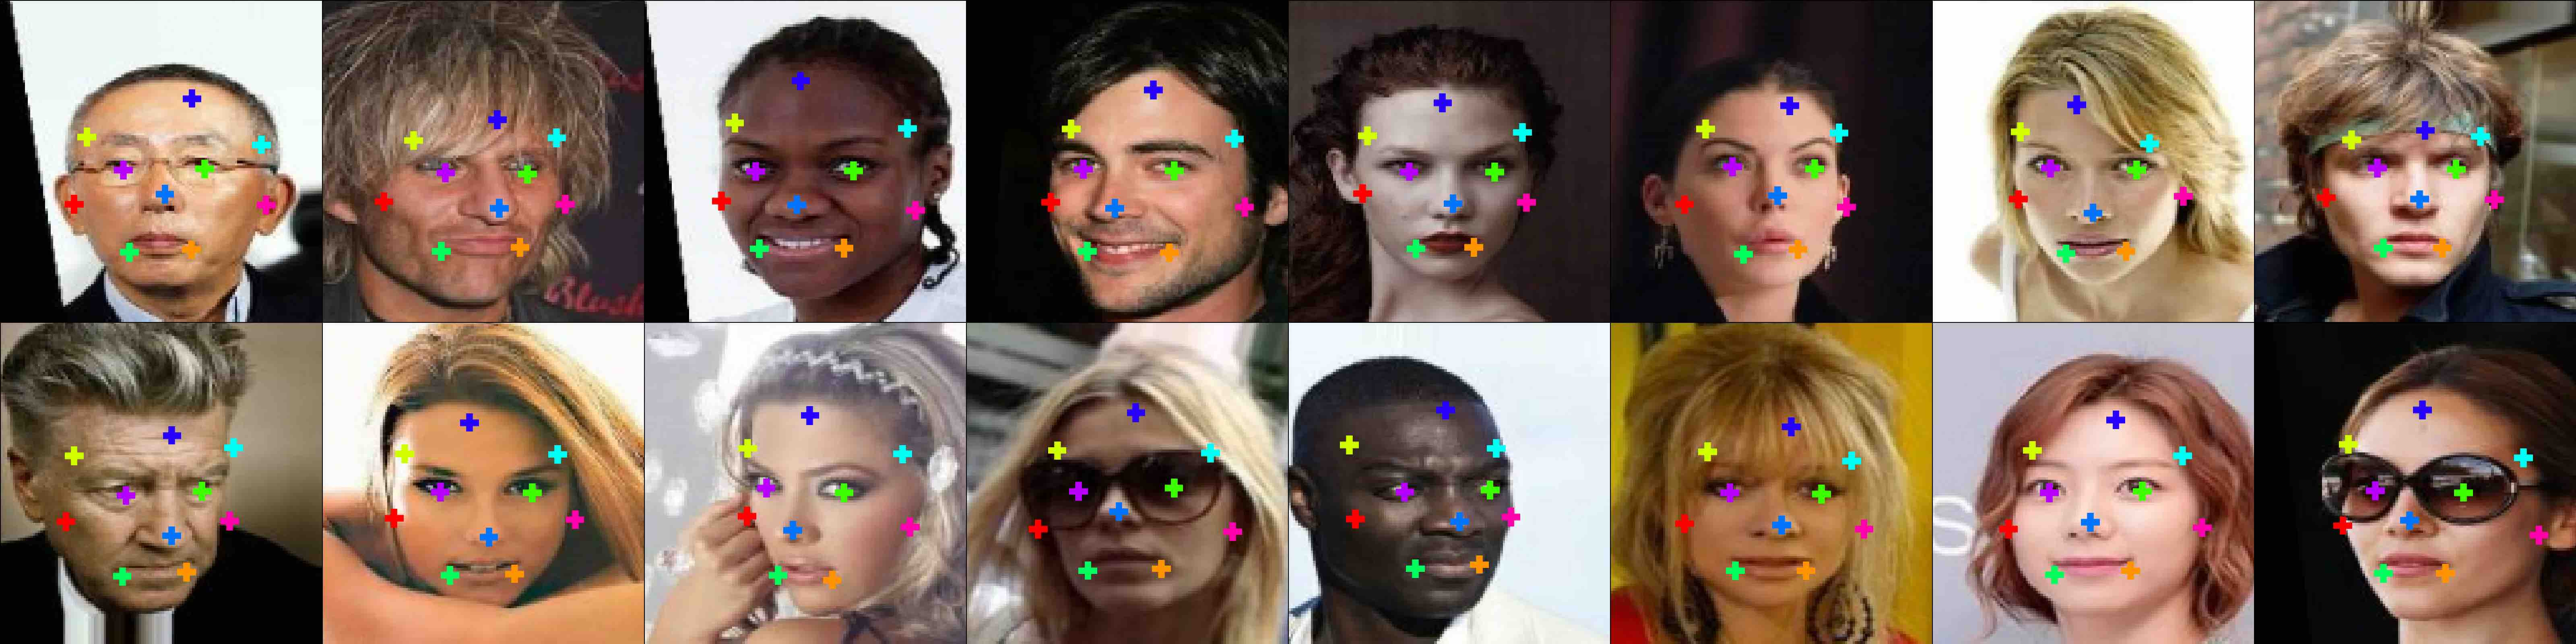
\includegraphics[trim={0cm 0cm 0cm 0cm},clip, width=1.\linewidth]{fig/shape/0celeba}\caption{}
			\end{subfigure}
			\begin{subfigure}{1.\textwidth}
			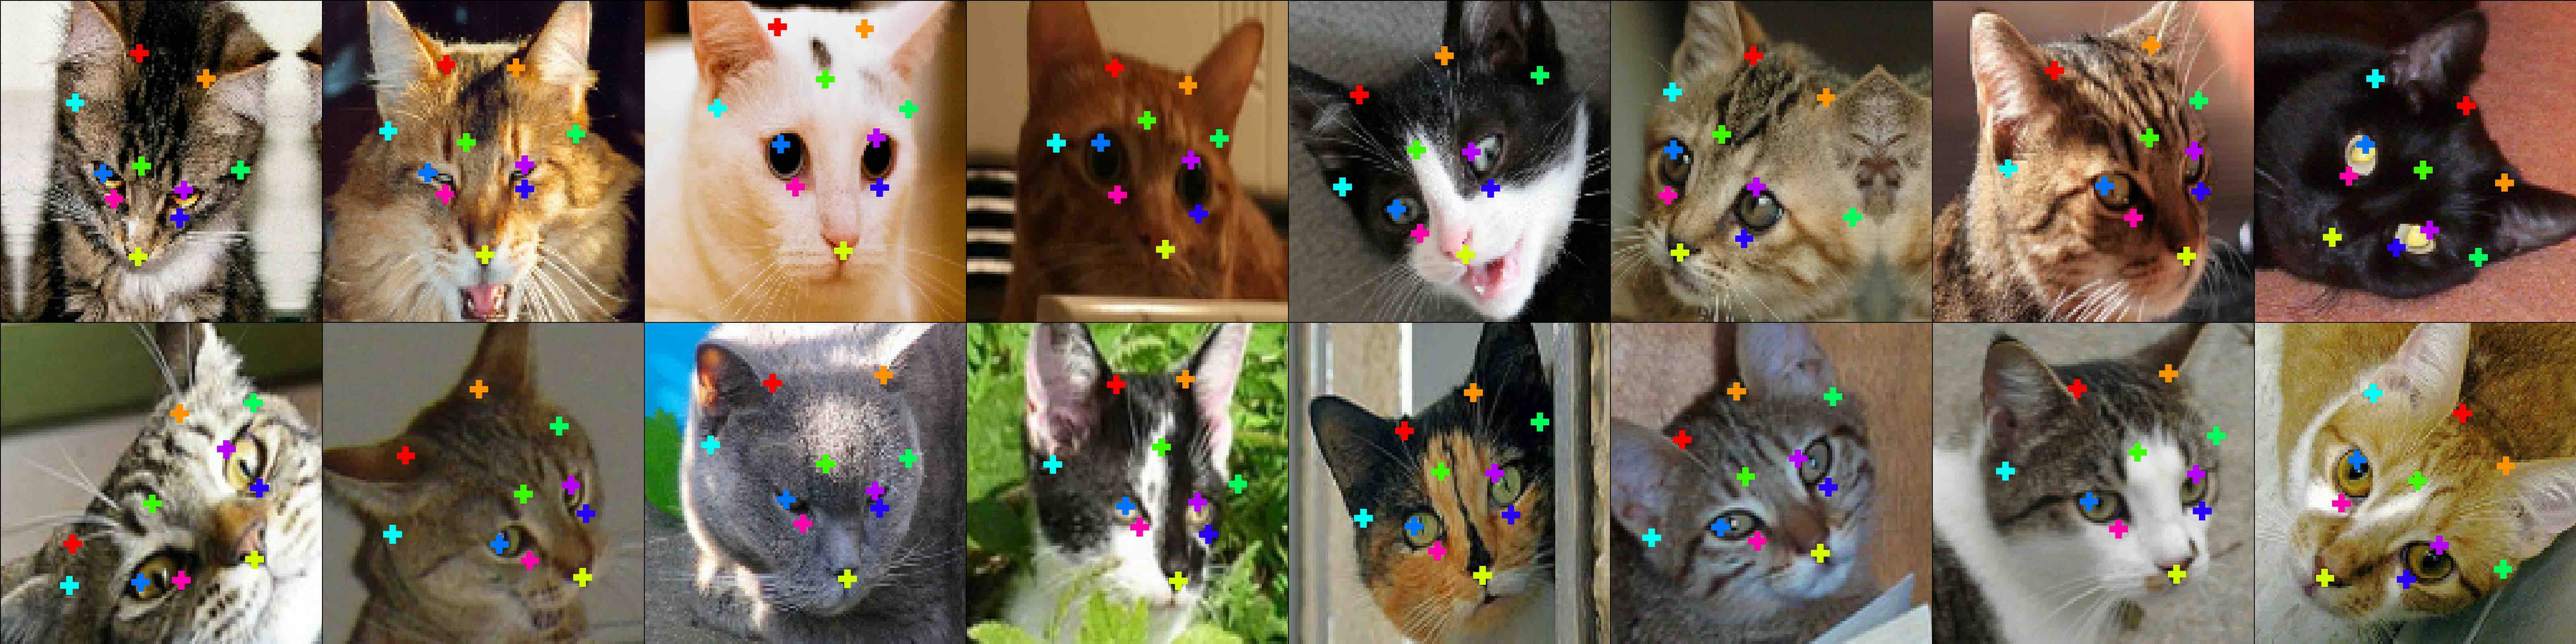
\includegraphics[trim={0cm 0cm 0cm 0cm},clip, width=1.\linewidth]{fig/shape/0cats}\caption{}
			\end{subfigure}
			\caption{{Unsupervised discovery of landmarks the object classes of (a) human (CelebA dataset) and (b) cat faces (Cat Head dataset).}}
			\label{fig:kp_faces}
		\end{figure}

		\subsubsection{Dataset preprocessing}
			\paragraph{CelebA} \cite{liu15facewild} contains ca. 200k celebrity faces of 10k identities.
			We resize all images to $128\times 128$ and exclude the training and test set of the MAFL subset, following \cite{thewlis17}.
			As  \cite{thewlis17, zhang18}, we train the regression (to 5 ground truth landmarks) on the MAFL training set (19k images) and test on the MAFL test set (1k images).

			\paragraph{Cat Head} \cite{zhang08cathead}  has nearly 9k images of cat heads.
			We use the train-test split of \cite{zhang18} for training (7,747 images) and testing (1,257 images).
			We regress 5 of the 7 (same as \cite{zhang18}) annotated landmarks.
			The images are cropped by bounding boxes constructed around the mean of the ground truth landmark coordinates and resized to $128\times128$.

		\subsubsection{Qualitative results}
			Due to different breeds, the Cat Head dataset exhibits large variations between instances. Cat faces feature more complicated texture and locally variant silhouettes \cite{zhang08cathead}, hence, require a better learning of both shape and appearance.

		\subsubsection{Quantitative results}
			% RESULTS FACES
			\begin{table}[t]
				\caption{Error of unsupervised methods for landmark prediction on the Cat Head, MAFL (subset of CelebA) testing sets. The error is in \% of inter-ocular distance.}
				\label{tab:faces}
				\centering
				\begin{tabular}{l|ccc}
				\hline
				Dataset & Cat Head &  & MAFL \\
				  \# Landmarks &10 & 20  & 10  \\
				  \hline
				 Thewlis \cite{thewlis17}
				 & 26.76 & 26.94 & 6.32    \\
				 Jakab \cite{jakab18}
				 & - & - & 4.69  \\
				 Zhang \cite{zhang18}
				 & 15.35 & 14.84 & 3.46  \\
				  Ours & \textbf{9.88}  & \textbf{9.30} & \textbf{3.24}  \\ \hline  % image length is 600: 32.15 , 23.51
				\end{tabular}
			\end{table}
			Tab.~\ref{tab:faces} compares against the state-of-the-art.
			Our approach outperform competing methods by a large margin, with particularly good performance on the more challenging Cat Head dataset.
	\subsection{Human Bodies}
		% BODIES
		\begin{figure}[htp]
			\centering
			\begin{subfigure}{1.\textwidth}
			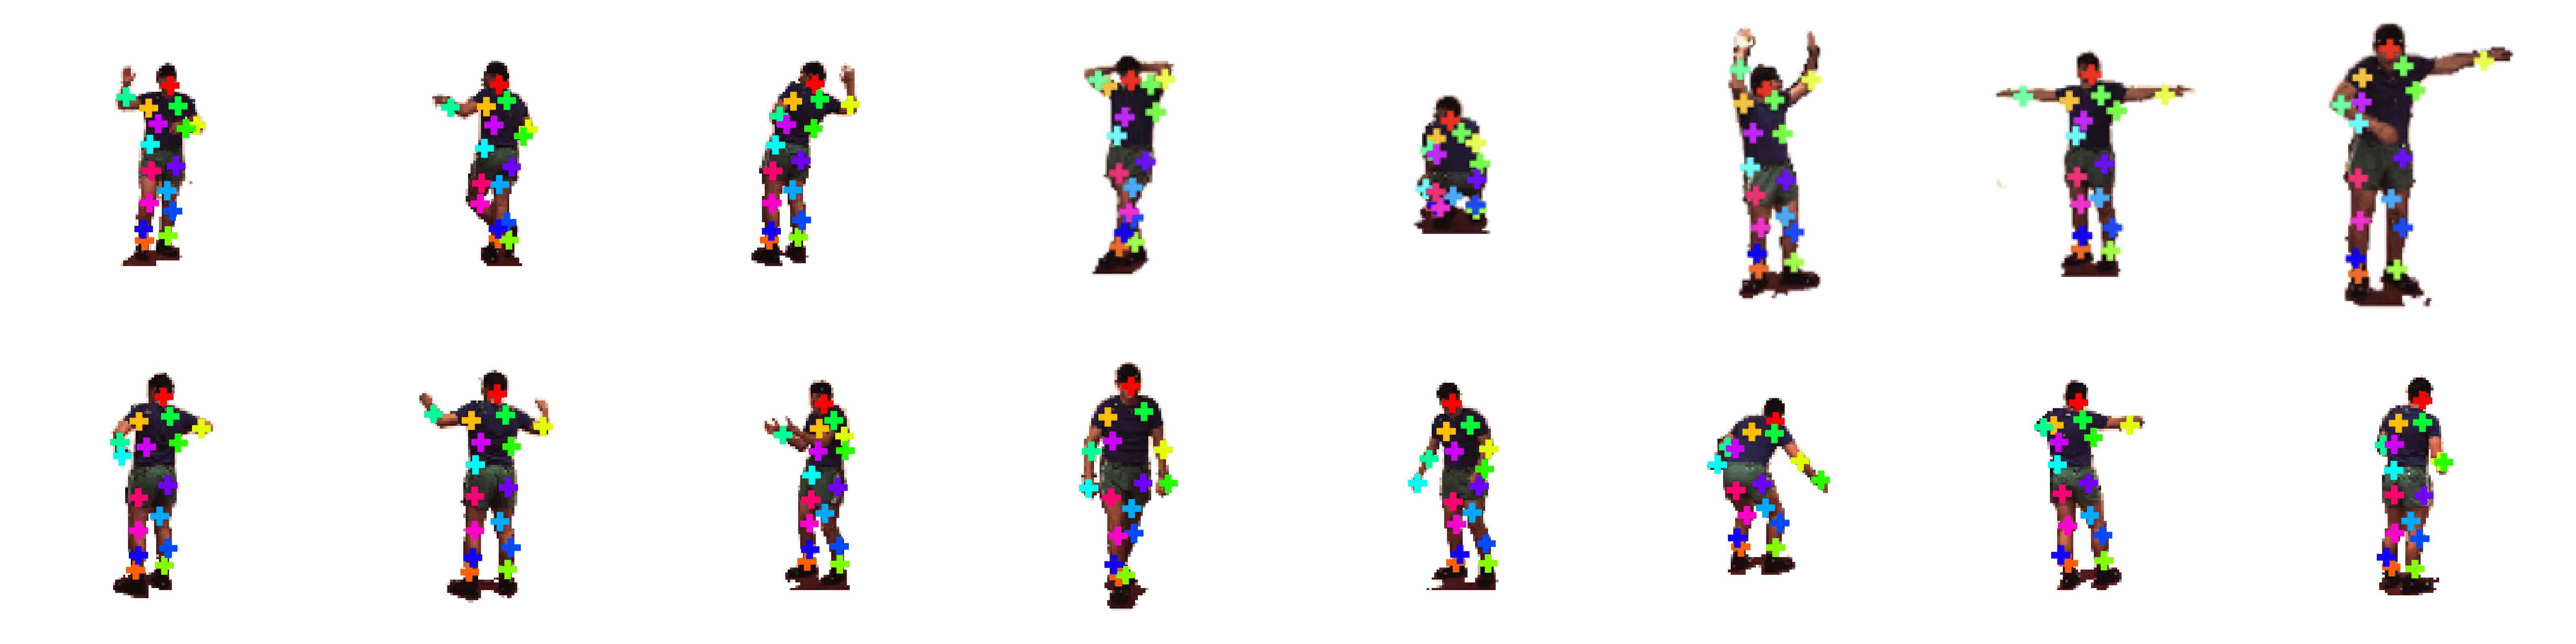
\includegraphics[trim={0cm 0cm 0cm 0cm},clip, width=1.\linewidth]{fig/shape/0human}\caption{}
			\end{subfigure}
			\begin{subfigure}{1.\textwidth}
			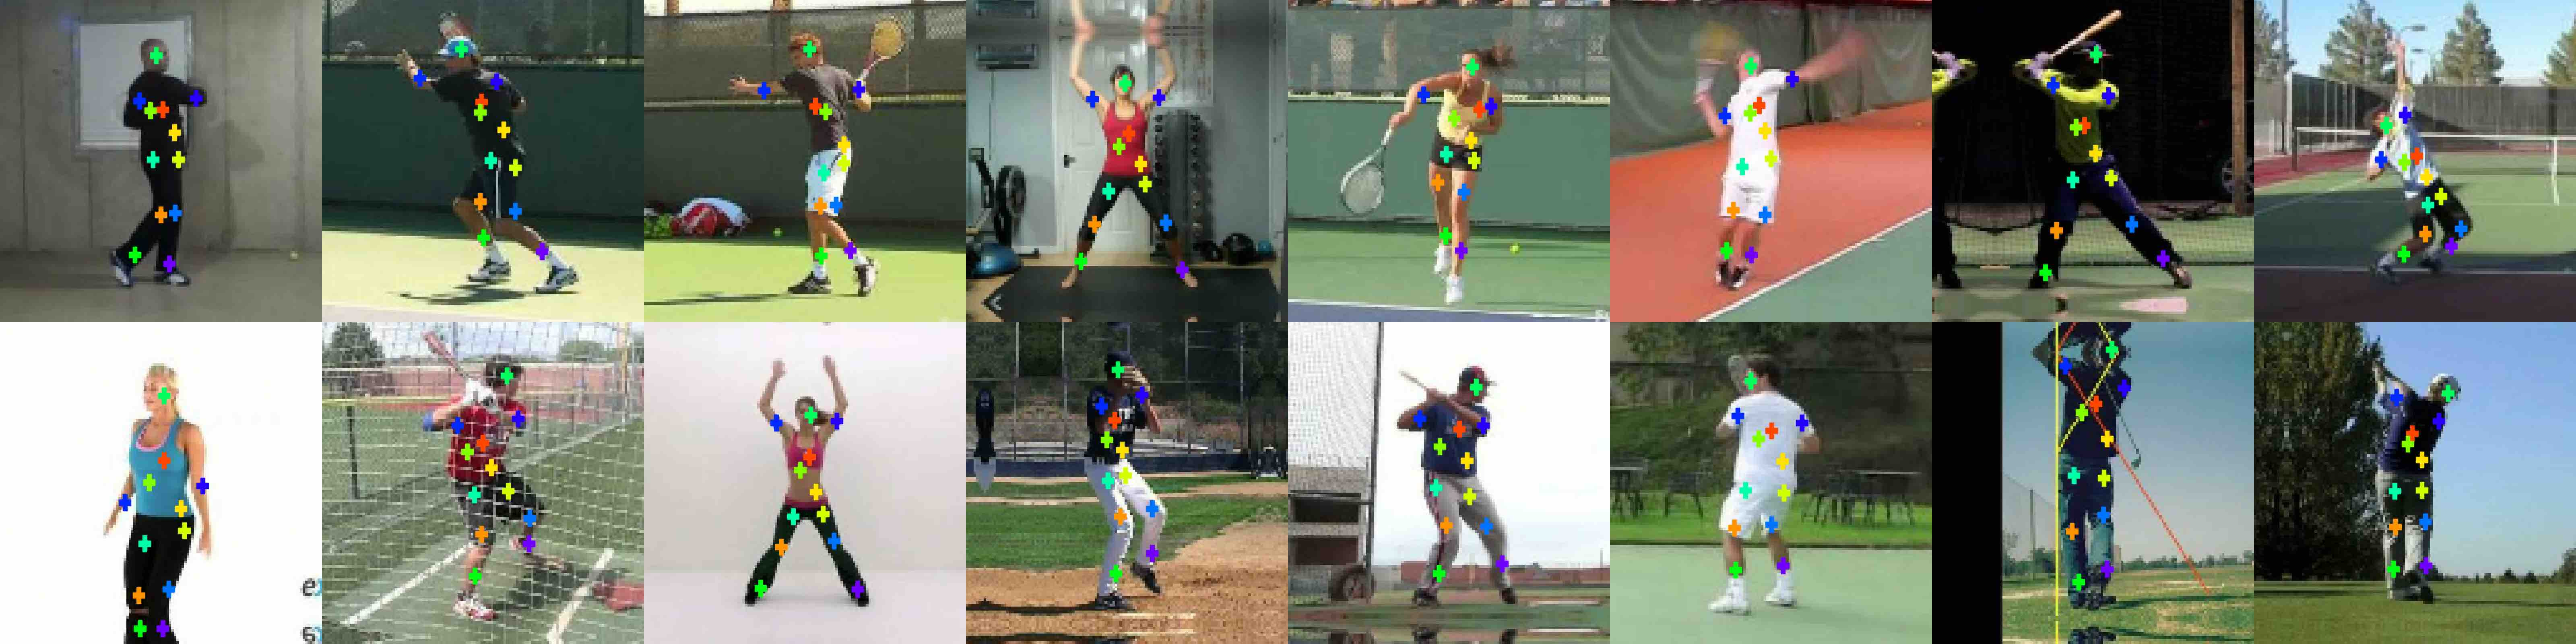
\includegraphics[trim={0cm 0cm 0cm 0cm},clip, width=1.\linewidth]{fig/shape/0penn}\caption{}
			\end{subfigure}
			\caption{{Unsupervised discovery of landmarks the object classes of human bodies (a) in constrained (Human3.6M dataset) and (b) unconstrained environments (Penn Action dataset).}}
			\label{fig:kp_bodies}
		\end{figure}

		\subsubsection{Dataset preprocessing}
			\paragraph{BBC Pose} \cite{charles13bbcpose} contains videos of sign-language signers with varied appearance in front of a changing background. Like \cite{jakab18} we loosely crop around the signers.
			The test set includes 1000 frames and the test set signers did not appear in the train set.
			For evaluation, as \cite{jakab18}, we utilized the provided evaluation script, which measures the PCK around $d=6$ pixels in the original image resolution.


			\paragraph{Human3.6M} \cite{ionescu14human36m} features human activity videos.
			We adopt the training and evaluation procedure of \cite{zhang18}.
			For proper comparison to \cite{zhang18} we also removed the background using the off-the-shelf unsupervised background subtraction method provided in the dataset.


			\paragraph{Penn Action} \cite{zhang13penn} contains 2326 video sequences of 15 different sports categories.
			For this experiment we use 6 categories (tennis serve, tennis forehand, baseball pitch, baseball swing, jumping jacks, golf swing).
			We roughly cropped the images around the person, using the provided bounding boxes, then resized to $128\times128$.

		\subsubsection{Qualitative results}
			We demonstrate (Fig. \ref{fig:kp_bodies}), that our model not only exhibits strong landmark consistency under articulation, but also covers the full human body meaningfully.
			Even fine-grained parts such as the arms are tracked across heavy body articulations, which are present in the Human3.6M or Penn Action datasets.
			Also with further complications such as viewpoint variations, blurred limbs and partial self-occlusions we are able to detect landmarks on Penn Action of similar quality and coverage as in the more constrained Human3.6M dataset.
			Additionally, complex background clutter, as in BBC Pose and Penn Action, does not hinder finding the object.

		\subsubsection{Quantitative results}
			% BBC POSE Results
			\begin{table}[htp]
				\caption{{
				Performance of landmark prediction on BBC Pose test set. As upper bound, we also report the performance of supervised methods.
				%Comparing against supervised and unsupervised methods for annotated landmark prediction on the BBC Pose testing set.
				The metric is \% of points within 6 pixels of groundtruth location. %Note that Jakab et al. are using a 50-landmarks, while we only use a 30 landmarks as input for the regression.
				}}
				\label{tab:bbcpose}
				\centering
				\begin{tabular}{ll|cr}
				\hline
				BBC Pose &   &    { Accuracy}  \\
				 \hline
				supervised & Charles \cite{charles13bbcpose} &
				   79.9\%  \\ % 79.90
				 & Pfister \cite{pfister15flowingconv}  &
				  88.0\%  \\ \hline % 88.01
				unsupervised &Jakab \cite{jakab18} &
				 68.4\%  \\  % 68.44
				  &Ours &  \textbf{74.5}\% \\
				% test pck = 0.7484605918670523
				% test pck_per_kp = [0.9633621  0.6627155  0.76508623 0.54956895 0.6928879  0.76616377   0.83943963]
				\hline
				\end{tabular}
			\end{table}

			% HUMAN3.6M Results
			\begin{table}[htp]
				\caption{{Comparing against supervised, semi-supervised and unsupervised methods for landmark prediction on the Human3.6M test set. The
				error is in \% of the edge length of the image. All methods predict 16 landmarks.
				}}
				\label{tab:human}
				\centering
				\begin{tabular}{ll|cr}
				\hline
				 Human3.6M   & &  { Error w.r.t. image size}  \\
				 \hline
				 supervised & Newell \cite{newell16hourglass}
				  &2.16  \\  \hline
				 semi-supervised & Zhang \cite{zhang18}
				  & 4.14  \\ \hline
				 unsupervised & Thewlis \cite{thewlis17}
				 & 7.51  \\
				  & Zhang \cite{zhang18}
					& 4.91 \\
				  & Ours& \textbf{2.79} \\
				\hline
				\end{tabular}
			\end{table}

			The quantitative results are shown in Tab. \ref{tab:bbcpose} and Tab. \ref{tab:human}: other unsupervised and semi-supervised methods are outperformed by a large margin on both datasets.
			On Human3.6M, judging by the performance gap, it is questionable whether the other unsupervised method from Thewlis \etal \cite{thewlis17} learned to deal with articulation at all.
			On Human3.6M, Zhang \etal \cite{zhang18} additionally used optical flow to stabilize their training, which we classified as semi-supervised, as using optical flow provides a significant information advantage.
			% On Human3.6M, our approach is able to achieve a large performance gain even over results obtained with optical flow supervision. %The  relative position and errors of our landmarks compared to the manually annotated landmarks are shown in Fig. \ref{fig:regress}.
			On BBC Pose, we outperform \cite{jakab18} by $6.1\%$, reducing the performance gap to supervised methods significantly.





	\subsection{Animal Bodies}
		% DOGS, BIRDS
		\begin{figure}[htp]
			\centering
			\begin{subfigure}{1.\textwidth}
			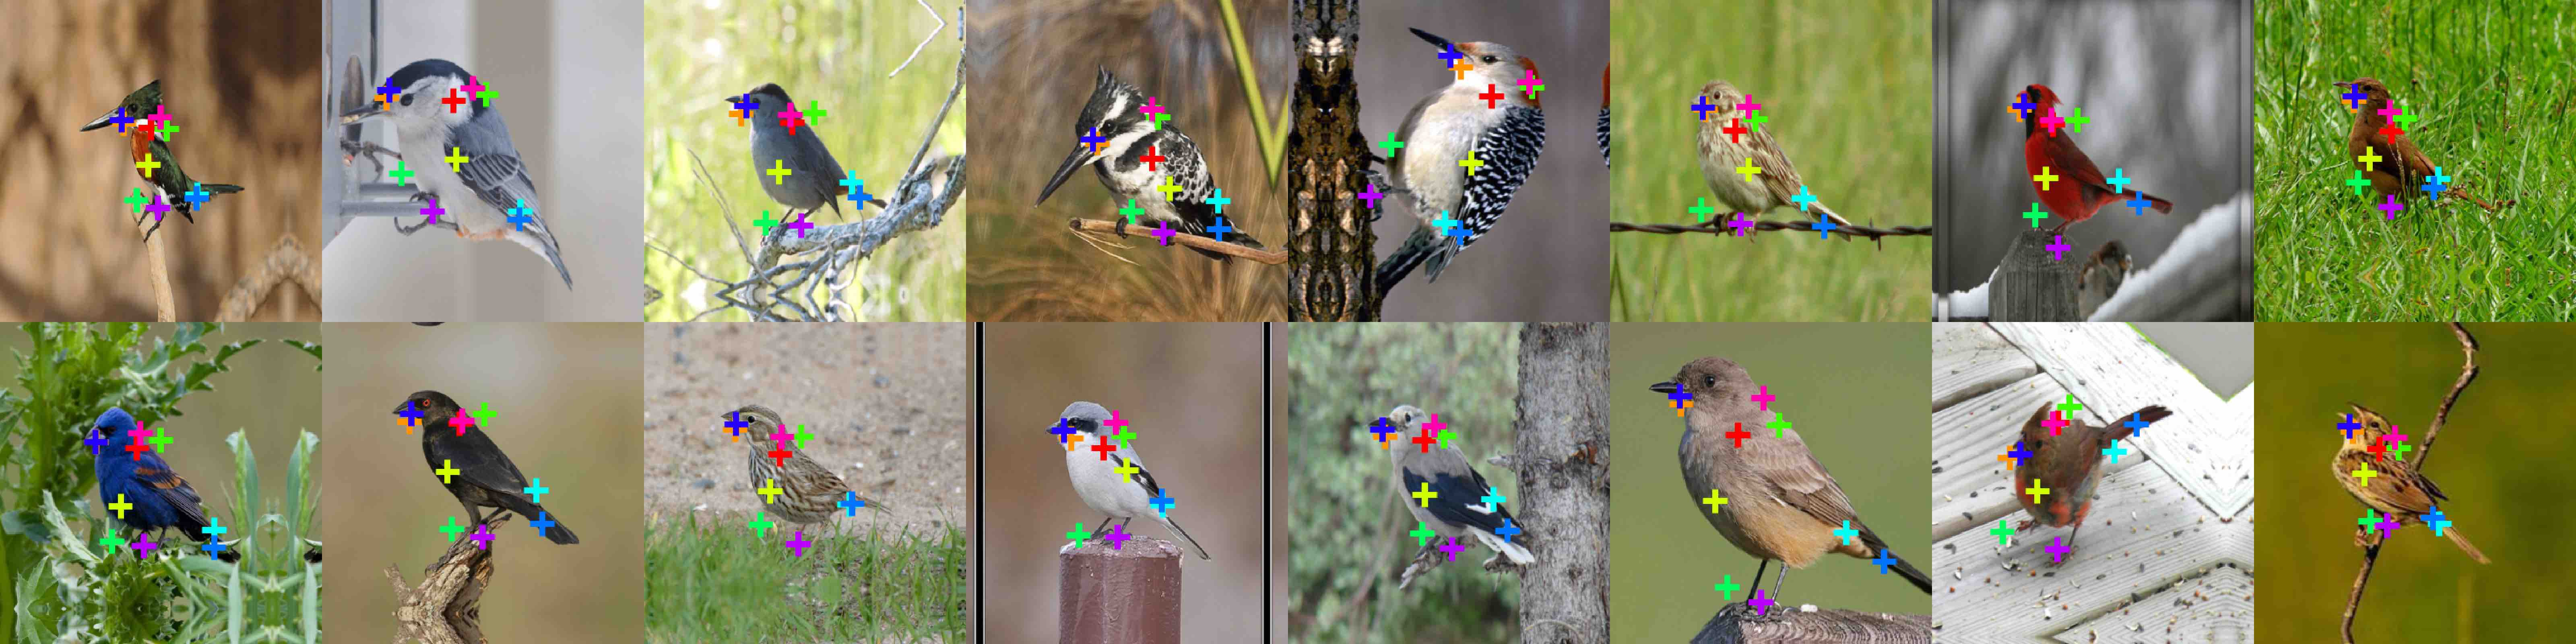
\includegraphics[trim={0cm 0cm 0cm 0cm},clip, width=1.\linewidth]{fig/shape/0birds}\caption{}
			\end{subfigure}
			\begin{subfigure}{1.\textwidth}
			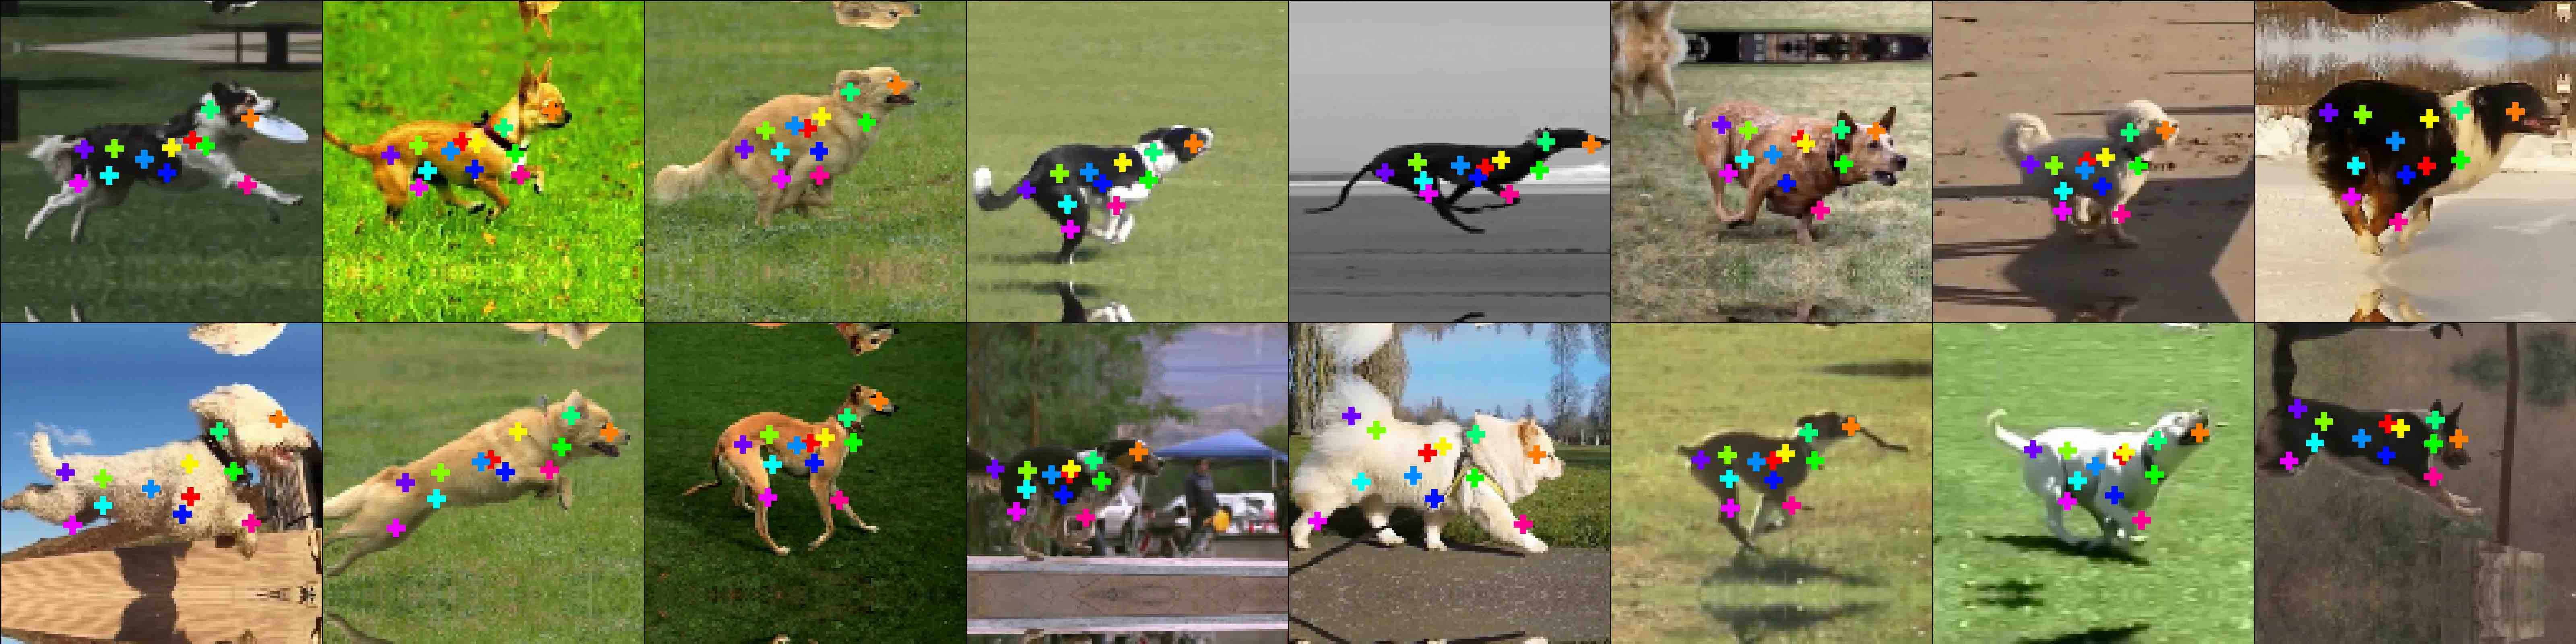
\includegraphics[trim={0cm 0cm 0cm 0cm},clip, width=1.\linewidth]{fig/shape/0dogs}\caption{}
			\end{subfigure}
			\caption{{Unsupervised discovery of landmarks the object classes of animal bodies (a) birds (CUB-200-2011 dataset) and (b) dogs (Dogs Run dataset).}}
			\label{fig:kp_animals}
		\end{figure}

		\subsubsection{Dataset preprocessing}
			\paragraph{CUB-200-2011} \cite{wah11birds} comprises ca. 12k images of birds in the wild from 200 bird species.
			We excluded bird species of seabirds, roughly cropped using the provided landmarks as bounding box information and resized to $128\times128$.
			We aligned the parity with the information about the visibility of the eye landmark.
			For comparing with \cite{zhang18} we used their published code.

			\paragraph{Dogs Run} is made from dog videos from YouTube totaling in 1250 images under similar conditions as in Penn Action. The dogs are running in one direction in front of varying backgrounds. The 17 different dog breeds exhibit widely varying appearances.

		\subsubsection{Qualitative results}
			The Dogs Run dataset displays that even completely different dog breeds can be related via semantic parts.
			Here, the universality of the approach (capturing non-human poses) is underlined once more.
			This is to be expected, as no prior assumptions about the object-class are introduced in the model.
			Furthermore, the limited amount of data in Dogs Run is no problem for finding meaningful correspondences, due to the unsupervised nature of the model and the transformations acting as a form of data augmentation.

		\subsubsection{Quantitative results}

			For a direct comparison to Zhang \etal \cite{zhang18} we apply their published code on the CUB-200-2011 dataset. The results are shown in Tab.~\ref{tab:birds}.

			% RESULTS BIRDS
			\begin{table}[t]
				\caption{Error of unsupervised methods for landmark prediction on the CUB-200-2011 testing set. Both methods predict 10 landmarks.}
				% The error is in \% of edge length of the image.}
				\label{tab:birds}
				\centering
				\begin{tabular}{l|cccc}
					\hline
					CUB-200-2011 dataset&  & Error \wrt image edge\\
					% \# Landmarks & 10  \\
					\hline
					Zhang \cite{zhang18} & 5.36 \\
					Ours  & \textbf{3.91}  \\ \hline
				\end{tabular}
			\end{table}

\end{comment}

\section{Challenges}\label{sec:challenges}
	%DATASET CHALLENGES
	\begin{table}
		\centering
		\caption{Difficulties of datasets: articulation, intra-class variance, background clutter and viewpoint variation}
		\label{tab:challenges}
		\begin{tabular}{l|rrrr}
			\hline
			Dataset &  Articul.& Var. &  Backgr.& Viewp.  \\ \hline
			CelebA &   &  &  &    \\
			Cat Head & &  \checkmark&  &   \\
			CUB-200-2011 & & \checkmark& \checkmark&   \\
			Human3.6M &\checkmark& &  & \checkmark  \\
			BBC Pose &  \checkmark&  & \checkmark&  \\
			Dogs Run & \checkmark& \checkmark& \checkmark&   \\
			Penn Action & \checkmark& \checkmark& \checkmark& \checkmark  \\
			\hline
		\end{tabular}
	\end{table}
	An overview over the challenges implied by each of the presented dataset is given in Tab.~\ref{tab:challenges}. We address the main difficulties in the following: background clutter~\ref{sec:background}, articulation~\ref{sec:articulation}, intra-class variance~\ref{sec:intraclass} and viewpoint variation~\ref{sec:viewpoint}.
	We discuss how the method overcomes these challenges.



	\subsection{Background Clutter}\label{sec:background}

		The question how to separate background from the object goes deeper than one might think. Fundamentally the question is: what is the object?
		For our algorithm the object is a common structure across all images which are presented to it. For it an object consists of parts which share a certain variance in feature space.

		If presented only images with birds sitting on twigs, the twig itself could as well be part of the object, couldn't it?

		dataset bias

		gaussian weighting (show image)

		prevent parts from explaining background, but

		What is an object? What is a scene? On a fundamental level, if only presented certain images with correlations to background \eg bird, twig, how to distinguish?
		compositional nature of reality
		Bird on twig object? Bird can also fly, but neural networks learn by correlation in data (-> ref to these failure modes)
		Dancing pair as object.
		human3.6m background too easy

		Complexly cluttered background - as long as no correlations to the object exist - is actually favorable for the method. Correlations of object with background will belong to object.

\begin{comment}
	\subsection{Object Articulation}\label{sec:articulation}
		Object articulation makes consistent landmark discovery challenging.
		Fig.~\ref{fig:kp_bodies} shows that our model exhibits strong landmark consistency under articulation and covers the full human body meaningfully.
		Even fine-grained parts such as the arms are tracked across heavy body articulations, which are frequent in the Human3.6M and Penn Action datasets.
		Despite further complications such as viewpoint variations or blurred limbs our model can detect landmarks on Penn Action of similar quality as in the more constrained Human3.6M dataset.
		% Additionally, complex background clutter as in BBC Pose and Penn Action, does not hinder finding the object.
		% Experiments on the Dogs Run dataset underlines that even completely dissimilar dog breeds can be related via semantic parts.
		% Tab.~\ref{tab:bbcpose} and Tab.~\ref{tab:human} summarize the quantitative evaluations: we outperform other unsupervised and semi-supervised methods by a large margin on both datasets.
		% On Human3.6M, our approach achieves a large performance gain even compared to methods that utilize optical flow supervision.
		% On BBC Pose, we outperform \cite{jakab18} by $6.1\%$, reducing the performance gap to supervised methods significantly.

	\subsection{Intra-Class Variation}\label{sec:intraclass}

		on cat head, human mislabelling is the most common failure mode

	\subsection{Viewpoint Variation}\label{sec:viewpoint}
		ill-posed fundamentally if reconstruction, cf.\ bbcpose to see that from trainset possible.
		especially difficult for CNNs~\cite{sabour17capsule}


\section{Analysis}
	\subsection{Transformations}\label{sec:transformations}
		\note{in this section: effect of transformations on learning, disentangling}
		\note{effectively connecting samples from the dataset, spreading the}
		\note{schedule transformations with exponential}

		\subsubsection{Parity}
			birds parity
			salsa parity

		\subsubsection{Rotation, Scaling, Translation}
			on Cats -> black cats different set of KP than rest -> connect these samples via transformation to reach intra-class consistency

		\subsubsection{Mimicking Appearance}
			% COLOR
			\begin{figure}[htp]
				\centering
				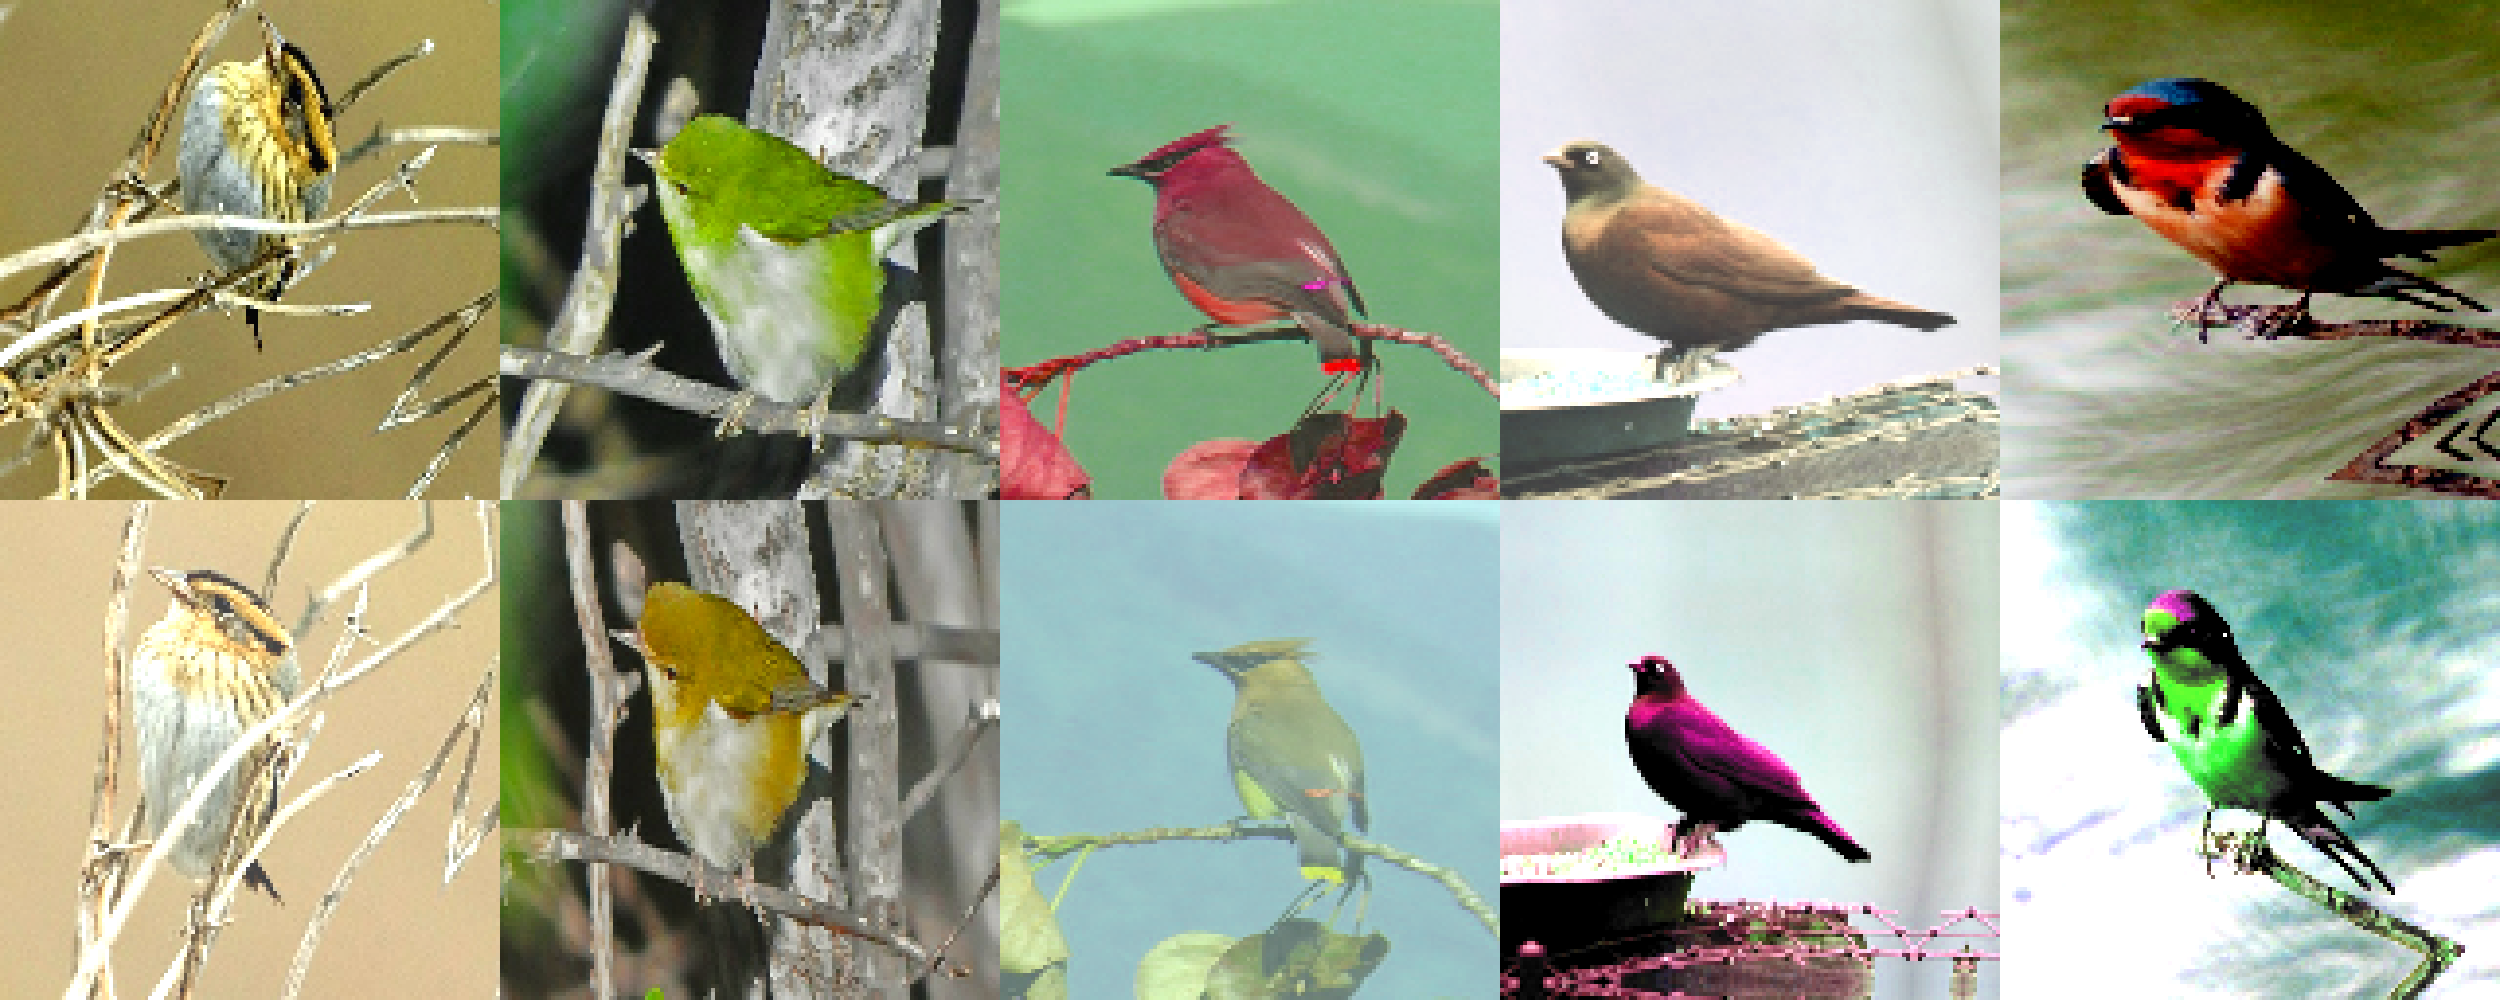
\includegraphics[trim={0cm 0cm 0cm 0cm},clip, width=.8\linewidth]{fig/shape/coloraugm}
				\caption{Examples for shape and appearance transformation on CUB-200-2011.}
				\label{fig:compare}
			\end{figure}


			Color, Contrast, Hue
			\subsection{Natural Changes in Video Data}
			Video data: Penn, Own

	\section{Comparative Advantages}
		\subsection{Non-Disentangling}
			% HUMAN3.6M DETAILED RESULTS
			\begin{table}[!ht]
				\centering
				\begin{tabular}{l|ccccccccr}
				\hline
				Dataset & Human3.6M &  &  &  & &  &  \\
				Actions & {\footnotesize All} & {\footnotesize Directions} & {\footnotesize Discussion} &  {\footnotesize Waiting }& {\footnotesize Greeting }& {\footnotesize Posing} & {\footnotesize Walking} \\
				\hline
				Newell \cite{hourglass} (supervised)
				&2.16 &1.88 &1.92 &2.15 &1.62 &1.88 &2.21 \\
				Zhang \cite{Zhang18}  (semi-supervised)
				& 4.14 & 5.01 & 4.61 & 4.76 & 4.45 & 4.91 & 4.61 \\  \hline
				Thewlis \cite{thewlis17}  (unsupervised)
				& 7.51 & 7.54 & 8.56 & 7.26 & 6.47 & 7.93 & 5.40 \\
				Ours (unsupervised) & \textbf{2.79} & \textbf{2.58} & \textbf{2.26} & \textbf{2.87} & \textbf{3.08} & \textbf{2.67} & \textbf{3.35}\\
				\hline
				\end{tabular}
				\caption{{Comparison with unsupervised, semi-supervised and supervised methods for annotated landmark prediction on the Human 3.6M testing sets for selected actions. The
				error is in \% regarding the edge length of the image. All methods predict 16 landmarks, from which the 32 ground truth landmarks are regressed.}}
				\label{tab:gtregressionhuman}
			\end{table}

			% COMPARE ZHANG
			\begin{figure}[htp]
				\centering
				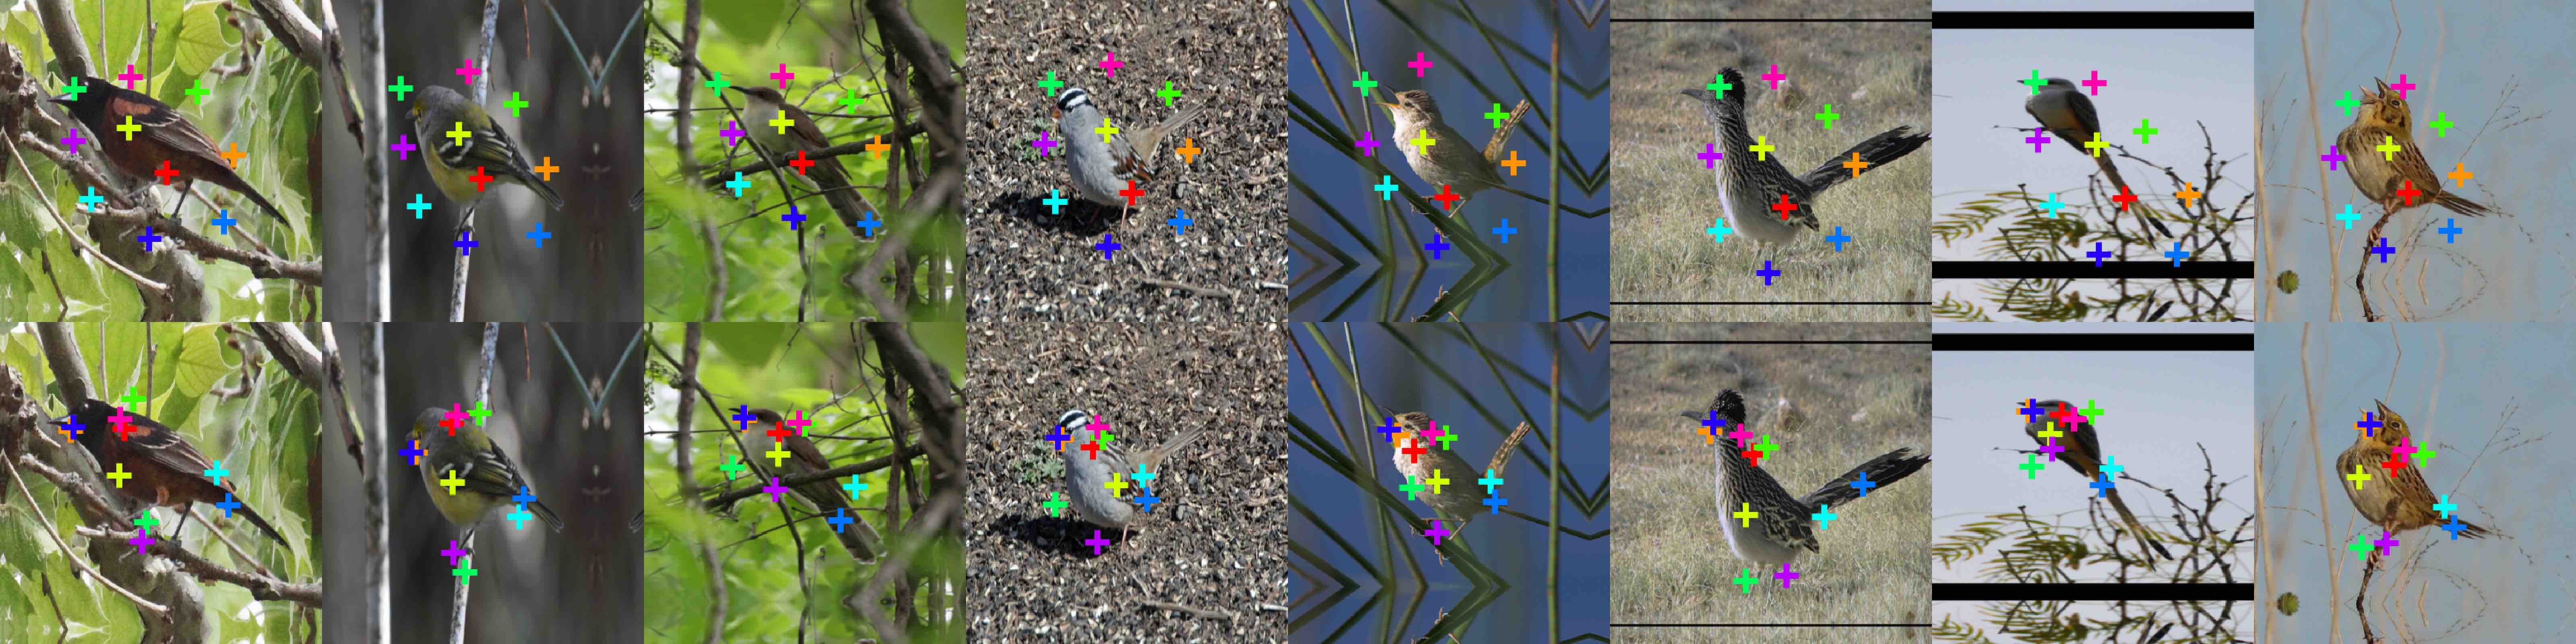
\includegraphics[trim={0cm 0cm 0cm 0cm},clip, width=1.\linewidth]{fig/shape/comp}
				\caption{Comparing discovered keypoints against \cite{zhang18} on CUB-200-2011. We improve on object coverage and landmark consistency. Note our flexible part placement compared to a rather rigid placement of \cite{zhang18} due to their part separation bias.}
				\label{fig:compare}
			\end{figure}

			Fig. \ref{fig:compare} provides a direct visual comparison to \cite{zhang18} on CUB-200-2011. It becomes evident that our predicted landmarks track the object much more closely. In contrast, \cite{zhang18} have learned a slightly deformable, but still rather rigid grid.
			This is due to their separation constraint, which forces landmarks to be mutually distant. We do not need such a problematic bias in our approach, since the localized, part-based representation and reconstruction guides the shape learning and captures the object and its articulations more closely.

		\subsection{Non-Factorizing}
			\begin{itemize}
				\item not factorizing into parts, holistic appearance
				\item disentangle via video
			\end{itemize}

			% BBCPOSE DETAILED RESULTS
			\begin{table}[!ht]
				\centering
				\begin{tabular}{l|ccccccr}
				\hline
				Dataset & BBCPose &  &  &  & &  &  \\
				Landmarks & {\footnotesize Head} & {\footnotesize Wrists} &  {\footnotesize Elbows }& {\footnotesize Shoulders } & {\footnotesize Avg.}  \\
				\hline
				Charles et al. \cite{charles}  (supervised)&
				95.40 & 72.95 & 68.70 & 90.30 & 79.90  \\
				Pfister et al.  \cite{pfister} (supervised) &
				98.00 & 88.45 & 77.10 & 93.50 & 88.01  \\ \hline
				Jakab \cite{jakab18}  (unsupervised) &
				76.10& 56.50& 70.70& 74.30 &68.44  \\
				Ours (unsupervised)  & \textbf{96.34} & \textbf{71.39} & \textbf{62.12} & \textbf{80.28}& \textbf{74.85} \\
				% test pck = 0.7484605918670523
				% test pck_per_kp = [0.9633621  0.6627155  0.76508623 0.54956895 0.6928879  0.76616377   0.83943963]
				\hline
				\end{tabular}
				\caption{{Comparison with supervised and unsupervised methods for annotated landmark prediction on the BBCPose testing sets.
				\%-age of points within d= 6-pixels of ground-truth is reported.}}
				\label{tab:gtregressionhuman}
			\end{table}

			%  COMPARISON TO JAKAB
			\begin{figure}[!ht]
				\centering
				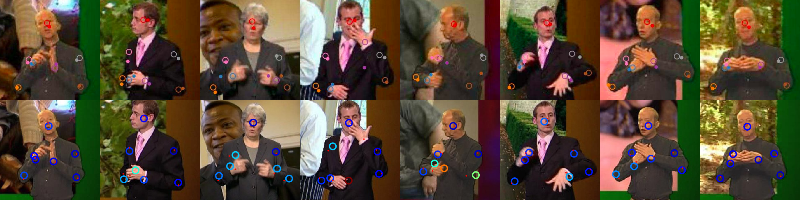
\includegraphics[trim={0cm 0cm 0cm 0cm},clip, width=1.\linewidth]{mat/bbc8}
				\caption{{Comparison of regression results of our method (bottom rows) to \cite{jakab18} (top rows) on BBC POSE. For visualization by Jakab \etal (from their paper) ground truth is in circles and the corresponding regression in the same color. For our visualization the red dots mark the ground truth, the colored circles the regressed locations. The color coding is in terms of the error \wrt the image edge length.}}
				\label{fig:bbc8}
			\end{figure}

	\subsection{Ablating Contributions}\label{sec:ablation}
		% ABLATION STUDY
		\begin{table}
			\centering
			\begin{tabular}{l|cr}
				\hline
				Dataset & Cat Head    \\
				\# Landmarks &  20 \\ \hline
				full model &  9.30 \\ \hline
				w/o $\mathcal{L}_{\textrm{eq}}$   & 11.32 \\
				w/o $\mathcal{L}_{\textrm{rec}}$   & 35.0 \\
				w/o appearance transform & 12.46 \\
				w/o shape transform & 14.72 \\ \hline
			\end{tabular}
			\caption{{Ablation studies on Cat Head dataset. We ablate the reconstruction loss $\mathcal{L}_{\textrm{rec}}$, equivariance loss $\mathcal{L}_{\textrm{eq}}$, the color augmentation and the crossing task}}
			\label{tab:ablation}
		\end{table}

		% what is the color augmentation: explain before
		\todo{what is the crossing task}
		We ablate the main components of our proposed framework: reconstruction loss $\mathcal{L}_{\textrm{rec}}$, the equivariance loss $\mathcal{L}_{\textrm{eq}}$, the appearance augmentation and the crossing task for disentangling shape and appearance. For the ablation study we use the Cat Head dataset, following the already introduced train-test setup on the task of landmark ground truth regression. Tab. \ref{tab:ablation} illustrates the ablation results.\\
		Leaving out the reconstruction task naturally leads to the largest drop in performance since only training on equivariance leads to collapsed landmark solutions as discussed in \cite{zhang18}.
		Training our model without color augmentations or appearance crossing between image pairs (i.e. the crossing task) weakens, respectively neglects the disentanglement of appearance and shape and hence the performance of our model significantly. % here specifically tackling intra-class variance
		Note that without the crossing task our models performs on par with Zhang \etal \cite{zhang18}, indicating, that this novel task could be explaining overall performance gain \wrt \cite{zhang18}. %This performance drop would be larger on datasets with articulation.
		Leaving out the explicit equivariance leads to the smallest drop in performance. This is not surprising, as equivariance is implicitly also enforced in the crossing framework.
		% without local features (not done yet, should we?, could ablate local decoder, or part appearance)

	\subsection{Crucial role of Transformations}
		The proposed method enables to abstract away object appearance from shape.
		Despite the multifarious challenges in the diverse range of datasets, the method is able to learn a dedicated part representation for shape.
		We compare to other approaches and reach state-of-the-art performance on the task of regressing human-annotated landmarks from the part representation.
		The key difference to the most competitive approach \cite{zhang18} is the emphasis on disentanglement via a crossed reconstruction with shape and appearance transformations.
		Enforcing disentanglement via targeted transformations enhances the shape representation in two ways: \emph{(i)} it asserts that no appearance information is encoded in the shape representation and vice versa and \emph{(ii)} it requires visual features to be equivariant under a spatial transformation.
		With regards to the considerations earlier, the crucial role of the transformations are to be expected, as they enable to reach a \textit{disentanglement}.
\end{comment}
